% This is "sig-alternate.tex" V2.1 April 2013
% This file should be compiled with V2.5 of "sig-alternate.cls" May 2012
%
% This example file demonstrates the use of the 'sig-alternate.cls'
% V2.5 LaTeX2e document class file. It is for those submitting
% articles to ACM Conference Proceedings WHO DO NOT WISH TO
% STRICTLY ADHERE TO THE SIGS (PUBS-BOARD-ENDORSED) STYLE.
% The 'sig-alternate.cls' file will produce a similar-looking,
% albeit, 'tighter' paper resulting in, invariably, fewer pages.
%
% ----------------------------------------------------------------------------------------------------------------
% This .tex file (and associated .cls V2.5) produces:
%       1) The Permission Statement
%       2) The Conference (location) Info information
%       3) The Copyright Line with ACM data
%       4) NO page numbers
%
% as against the acm_proc_article-sp.cls file which
% DOES NOT produce 1) thru' 3) above.
%
% Using 'sig-alternate.cls' you have control, however, from within
% the source .tex file, over both the CopyrightYear
% (defaulted to 200X) and the ACM Copyright Data
% (defaulted to X-XXXXX-XX-X/XX/XX).
% e.g.
% \CopyrightYear{2007} will cause 2007 to appear in the copyright line.
% \crdata{0-12345-67-8/90/12} will cause 0-12345-67-8/90/12 to appear in the copyright line.
%
% ---------------------------------------------------------------------------------------------------------------
% This .tex source is an example which *does* use
% the .bib file (from which the .bbl file % is produced).
% REMEMBER HOWEVER: After having produced the .bbl file,
% and prior to final submission, you *NEED* to 'insert'
% your .bbl file into your source .tex file so as to provide
% ONE 'self-contained' source file.
%
% ================= IF YOU HAVE QUESTIONS =======================
% Questions regarding the SIGS styles, SIGS policies and
% procedures, Conferences etc. should be sent to
% Adrienne Griscti (griscti@acm.org)
%
% Technical questions _only_ to
% Gerald Murray (murray@hq.acm.org)
% ===============================================================
%
% For tracking purposes - this is V2.0 - May 2012

\documentclass{sig-alternate-05-2015}
\usepackage{amsmath}
%\usepackage{algorithm}
\usepackage{algorithm2e}
\usepackage[noend]{algpseudocode}
\usepackage{eurosym}

\begin{document}


% Copyright
%setcopyright{acmcopyright}
%\setcopyright{acmlicensed}
\setcopyright{rightsretained}
%\setcopyright{usgov}
%\setcopyright{usgovmixed}
%\setcopyright{cagov}
%\setcopyright{cagovmixed}


\title{{Using Machine Learning to Set Exchange Rates for Medium Term Contracts}
}
\numberofauthors{2} 
\author{
\alignauthor
Eduardo Lorie\\
       \affaddr{Georgia Institute of Technology}\\
       \email{edlorie@gatech.edu}
\alignauthor 
Matthew Robinson \\
       \affaddr{Georgia Institute of Technology}\\
       \email{mrobinson72@gatech.edu}
}

\date{20 February 2016}

\maketitle

\section{Introduction}
International business involves considerable risk. This is especially true for manufacturers, who often make production decisions well in advance of delivery dates. Consider the position of an airline that is preparing to expand its fleet. Such an airline might place an order for a passenger jet that will not be completed for a year or more, with payment due upon delivery of the jet. If the buyer is American and the manufacturer is also American, this is not a problem. All of the manufacturers production costs will be valued in US dollars, and the customer will pay in US dollars.
\par{} In contrast, consider the situation if the buyer is Canadian and the manufacturer is American. Since the manufacturer is American, the Canadian firm must pay for the jet in US dollars. Suppose the value of the US dollar appreciates 10\% relative to the Canadian dollar while the American firm is filling the order. Then, when the Canadian firm pays for the jet, it is 10\% more expensive in terms of Canadian dollars than when it ordered it. If the movement were in the opposite direction, the manufacturer would receive 10\% fewer US dollars for the jet than it expected when it was ordered. Clearly, both firms would be interested in predicting adverse currency movements in advance, and may be interested in writing expected future currency valuations into contracts. 
\par{} In order to resolve this dilemma, we estimate several models that predict the percent change in the exchange rate after one year, using only information that is currently available. The predictors for these models include the current exchange rate, the interest rate, inflation rate and government bond yield for both countries, and several variables related to international trade and financial flows. The remainder of this section will provide an overview of relevant economic theory, a summary of past statistical research on exchange rates and an overview of the data set. In the following section, we perform exploratory data analysis to develop a basic understanding of the trends in the data set. Next, we develop several models for predicting exchange rates and compare their effectiveness. Finally, we conclude by suggesting the most effective means to predict exchange rates and possible directions for future research.

\subsection{Related Work}
Research on equilibrium in foreign exchange markets is a well developed component of classical economic theory. Classical models rest on two fundamental ideas. The first is that foreign exchange markets achieve equilibrium when the rate of return on deposits is the same across all currencies. The idea that investors will be indifferent between bank deposits denominated in different currencies is known as interest rate parity. The second is that the price of goods will be the same when valued in different currencies. The notion that a basket of goods should cost the same in all currencies is known as purchasing power parity.
\par{} Both of these concepts rely on the same basic premise, which is that price differentials create arbitrage opportunities. Interest rate and purchasing power parity hold that price differentials are self-correcting because, as investors move to take advantage of arbitrage opportunities, they push the market back toward equilibrium. To demonstrate this idea, suppose that a laptop costs \$500 in the United States and the Euro equivalent of \$550 in Germany. Someone in Germany could take advantage of this fact by buying cheap laptops in the US and selling them in Germany. This would create more demand for dollars, which are required to buy the laptops in the US, and push up US price levels. This trend would continue until price levels are high enough that laptops cost the same in the US as in Germany. When laptop prices are the same in both countries, the market is in equilibrium since there is no longer an opportunity for arbitrage.
\par{} The following equations summarize the relationship between exchange rates and interest rates under interest rate parity and the relationship between exchange rates and price levels under purchasing power parity, all else held equal. In these equations, $e_{t}$ represents the exchange rate at time $t$ in terms of the foreign currency, $i$ is the real interest rate and $\pi$ is the inflation rate. 
\begin{equation}
e_{t+1} = e_{t} \left( \frac{1+i_{d}}{1+i_{f}} \right)
\end{equation}
\begin{equation}
\frac{e_{t+1}-e_{t}}{e_{t}} = \frac{1+\pi_{d}}{1+\pi{f}} - 1
\end{equation}
\par{} Obstfeld and Taylor show that arbitrage opportunities between foreign and domestic assets are near zero under floating currency regimes, which suggests that exchange rates behave as predicted by interest rate parity. Likewise, Frankel and Rose provide evidence that exchange rates converge to levels predicted by purchasing power parity in the long run. The relevant time-frame for the \emph{long run} in this context is about four years. Under shorter time horizons, purchasing power parity performs considerably less well. Likewise, difficulty in predicting the relative performance of financial assets in different countries makes it difficult to predict interest rates using interest rate parity. In fact, Meese and Rogoff famously demonstrated that a random walk outperforms structural models for the exchange rate over a one to twelve month window. For this reason, the random walk is currently used as a benchmark for assessing the quality of models for predicting exchange rates.
\par{} Apart from random walks other approaches to have been studied to accurately determine future changes in exchange rates. Hsiech showed that there is little linear dependence in exchange-rate changes but there is a strong nonlinear dependence. On the other hand, Meese and Rose showed that nonlinear estimators to do not significantly improve popular models for predicting exchange rates. All these observations happened with the use of macroeconomic variables such as interest rates and inflation rates. Lyons and Evans showed that models become much more accurate with the introduction of microeconomics. They augmented previously used linear models with a new variable, order flow, which is the net of buyer and seller initiated orders. The introduction of this variable resulted in accurately predicting 60\% of daily changes in Deutsche mark/US dollar rate. 
\par{} Another popular model in determining future exchange rates is the artificial neural network. Panda and Narasimhan showed that Neural networks outperform both random walk and linear autoregressive models when predicting weekly changes in Indian rupee/US dollar exchange rates.   

\subsection{Data}
This paper restricts its attention to changes in the exchange rate between the United States and its five biggest trading partners, excluding China. These trading partners are Europe, Canada, Mexico, Japan and South Korea. Europe in this context refers to the 19 countries that belong to the eurozone. Since they have a single monetary policy, they will be treated as a single unit for the purposes of this paper. China is excluded because it fixes its exchange rate. Because of this, its exchange rate is determined by government policy rather than economic variables.
\par{} The data used in this paper was collected entirely by central banks and compiled by Quandl, an economic data repository. The primary variables of interest in the data set are the inflation rate, interest rate and the yield on one year government bonds. In this data set, the inflation rate measures the annualized percent change in the consumer price index for each country. The interest rate is the interbank lending rate set by the central bank for the currency in question. For the United States, this is the federal funds rate.  Other variables in the data set include an area's balance of trade, current account, foreign exchange reserves and other factors related to international financial flows. These variables were measured both for the United States and each currency pairing. Each variable is measured monthly, with the exception of GDP growth, current account balance and foreign direct investment. These variables are measured quarterly. In order to align this data with the rest of the data set, values for the intervening two months between each quarter were interpolated using cubic splines.

\section{Exploratory Data Analysis}

\subsection{Tests for Autocorrelation}
Time series data often exhibits autocorrelation. Autocorrelation refers to correlation between values of a variable at different points in time. In order to assess the degree of autocorrelation in the exchange rate data set, we fit a simplified linear model that consisted of the current exchange rate, along with the interest rate, inflation rate and government bond yield for both countries. After fitting the model, we computed the Durbin-Watson test statistic with one to twelve month lags. Figure~\ref{fig:autocorrelation} depicts the value of the correlation coefficient for each country as a function of time.
\par{} The test statistics show that the data set exhibits strong autocorrelation for several months, and that the severity of the autocorrelation decays over time. For each country, the correlation coefficient for a one month lag is in excess of 0.80, and is as high as 0.95 for Japan. This value drops below 0.50 for every country by month four, with the exception of Japan. The persistence of autocorrelation in the case of Japan may be due to its active currency manipulation policy. For each country, the correlation coefficient remains statistically significant for at least five months. The presence of autocorrelation in the data set argues for including lagged variables in the model, through at least several months.

\begin{figure}
\centering
\caption{Severity of Autocorrelation}
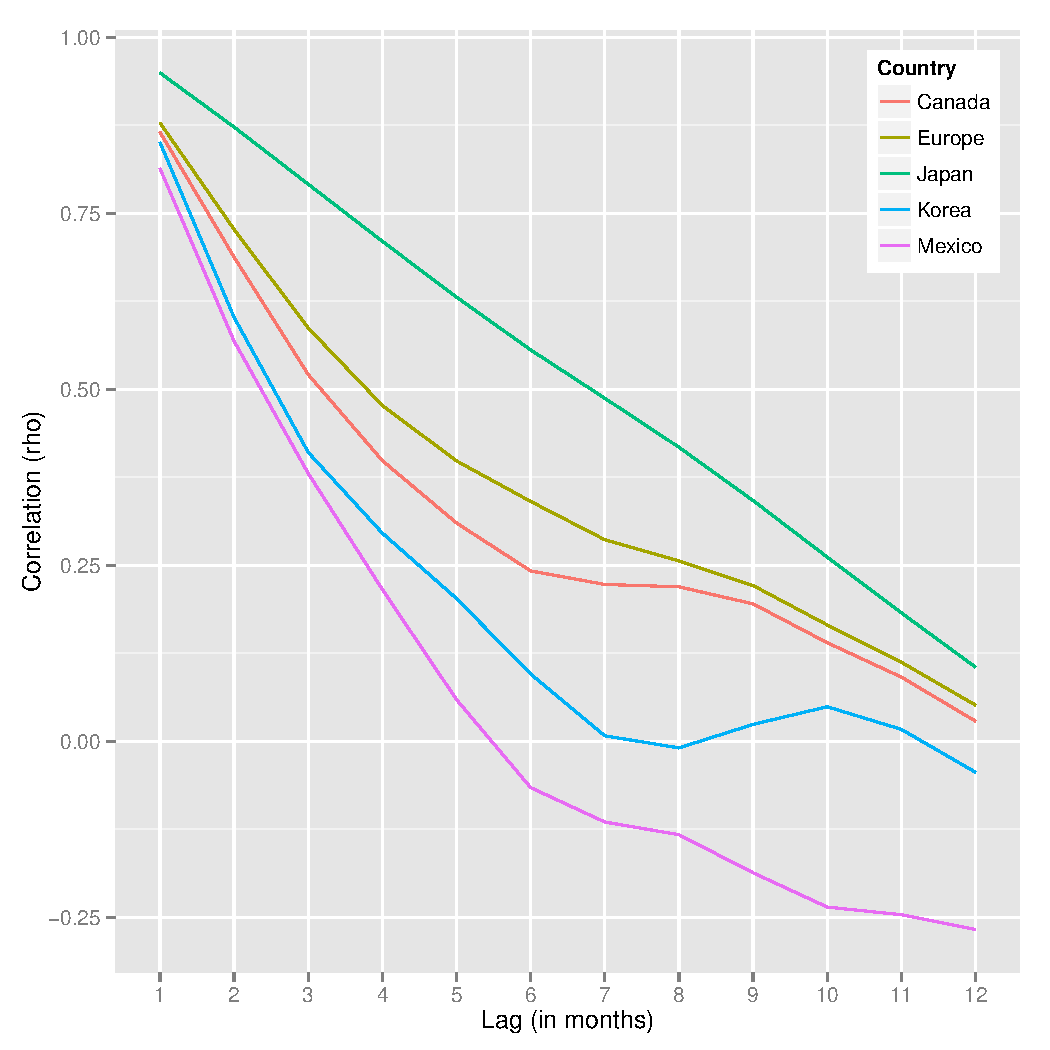
\includegraphics[scale=0.55]{autocorrelation.pdf}
\label{fig:autocorrelation}
\end{figure}

%\begin{figure}
%\centering
%\caption{Durbin-Watson Test -- Canada}
%\begin{tabular}{c c c c}
%Lag & Autocorrelation & D-W Statistic & p-value \\
%1 & 0.8421 & 0.2975 & 0.000 \\
%2 & 0.6337 & 0.6994 & 0.000 \\
%3 & 0.4381 & 1.0782 & 0.000 \\
%4 & 0.2848 & 1.3816 & 0.000 \\
%5 & 0.1718 & 1.6064 & 0.014 \\
%6 & 0.0814 & 1.7851 & 0.254 \\
%\end{tabular}
%\end{figure}

%\begin{figure}
%\centering
%\caption{Durbin-Watson Test -- Japan}
%\begin{tabular}{c c c c}
%Lag & Autocorrelation & D-W Statistic & p-value \\
%1 & 0.9314 & 0.1370 & 0.000 \\
%2 & 0.8477 & 0.3041 & 0.000 \\
%3 & 0.7660 & 0.4671 & 0.000 \\
%4 & 0.6799 & 0.6388 & 0.000 \\
%5 & 0.5959 & 0.8048 & 0.000 \\
%6 & 0.5164 & 0.9615 & 0.000 \\
%\end{tabular}
%\end{figure}

\section{Methods}
Constructing a model to predict exchanges requires the consideration of three important factors: which variables to include in the model, candidate methods for estimating the model and the criteria for evaluating each method. The variable selection process involves deciding which economic factors to include in the model, as well as how many months of lagged observations to include for each factor. Candidate methods were chosen by considering several statistical techniques with properties that made them appealing for the exchange rate data set. Finally, a method for evaluating the candidate solutions that accounts for autocorrelation in the data set is developed.

\subsection{Variable Selection}
Selecting which variables to include in the model requires deciding which economic factors are relevant and for how many months prior to the current observation. To recap, the variables in the data set include the current exchange, interest, inflation and GDP growth rates, as well as several variables related to international financial flows. There is a strong theoretical justification for including each of these variables in the model. Nevertheless, overfitting is potentially problematic due to the small size of the data set, especially after the inclusion of lagged variables. The proper lag was selected by comparing the performance of a linear regression model across a variety of lag values. For each lag value, the variables were chosen by forward stepwise variable selection, using AIC as the selection criteria. Specifying the model in this manner allows us to balance the trade off between training error and model complexity.

\subsection{Method Evaluation}
Evaluating the effectiveness of the candidate solution required splitting the data into training and test sets. In all cases described in this paper, the training set consists of 80\% of the available data, with the remaining allocated to the test set. In order to effectively form the training and test sets, two aspects of the data required consideration: autocorrelation and the size of the data set.
\par{} As discussed above, the data set used in this paper exhibits autocorrelation that remains significant for at least several months. Since the economic variables in the data set are heavily correlated over time, this means that the data set cannot be split between training and test sets simply by separating the data randomly. To illustrate the nature of the problem, suppose that an observation from May 2012 is randomly assigned to the training set and an observation from June 2012 is randomly assigned to the test set. Since the May and June observations are correlated, a model that overfits the training data might perform artificially well on the test set because the training set contains observations that are similar to observations in the test set. In order to circumvent this problem, the test set was chosen by selecting a continuous block of time with a random start date. Additionally, six months of data before and after the test block was discarded. This data was used in neither the training nor the test set in order to ensure that the observations in the test set were as independent as possible from the observations in the training set.
\par{} Since this paper considers monthly data, the number of observations in each time series is on the order of hundreds, ranging from 121 for Mexico to 459 for Japan. Due to the relatively low number of observations in the data set, a true appraisal of the effectiveness of each method requires an evaluation of its performance over a large number of random partitions. In order to accomplish this, we randomly selected 100 start points for each data set and computed the training error for each method at each start point. The same 100 start points were used for each method. This allows us to test the hypothesis that one method outperforms another by conducting pairwise two sample statistical tests. Using many randomly selected start dates has the added advantage of providing more variability for the test sets. Since continuous blocks of time are correlated, the peculiarities of a particular block of time may provide a distorted view of the effectiveness of a given method if only one block of time is used. As a result, using a continuous block of time with many randomly selected start points is a reasonable method for splitting the data between training and test sets.

\section{Results}

\subsection{Determining the Optimal Lag}
The lag was determined by considering the performance of a standard linear regression model with a variety of lags. Since we want the simplest model specification that provides accurate predictions, we choose the point at which including an additional month of lag stops improving the performance of the model. This is accomplished by plotting the mean training error of the model as a function of the lag. These plots appear in Figures ~\ref{fig:lag1} and ~\ref{fig:lag2}. The optimal lag values vary by country. Noticeable improvements in the performance of the model cease after month four for Canada and month five for Mexico. The results justify including lagged variables out to nine months for Europe, Japan and Korea. In the case of Korea, the decision to include a lengthy lag on the variables is less clear cut, since the model also performs well with shorter lags. However, the mean testing error decreases by a factor of two after the ninth month is included, making the increased complexity of the model worthwhile.

\begin{figure}
\centering
\caption{Model Performance for Various Lags}
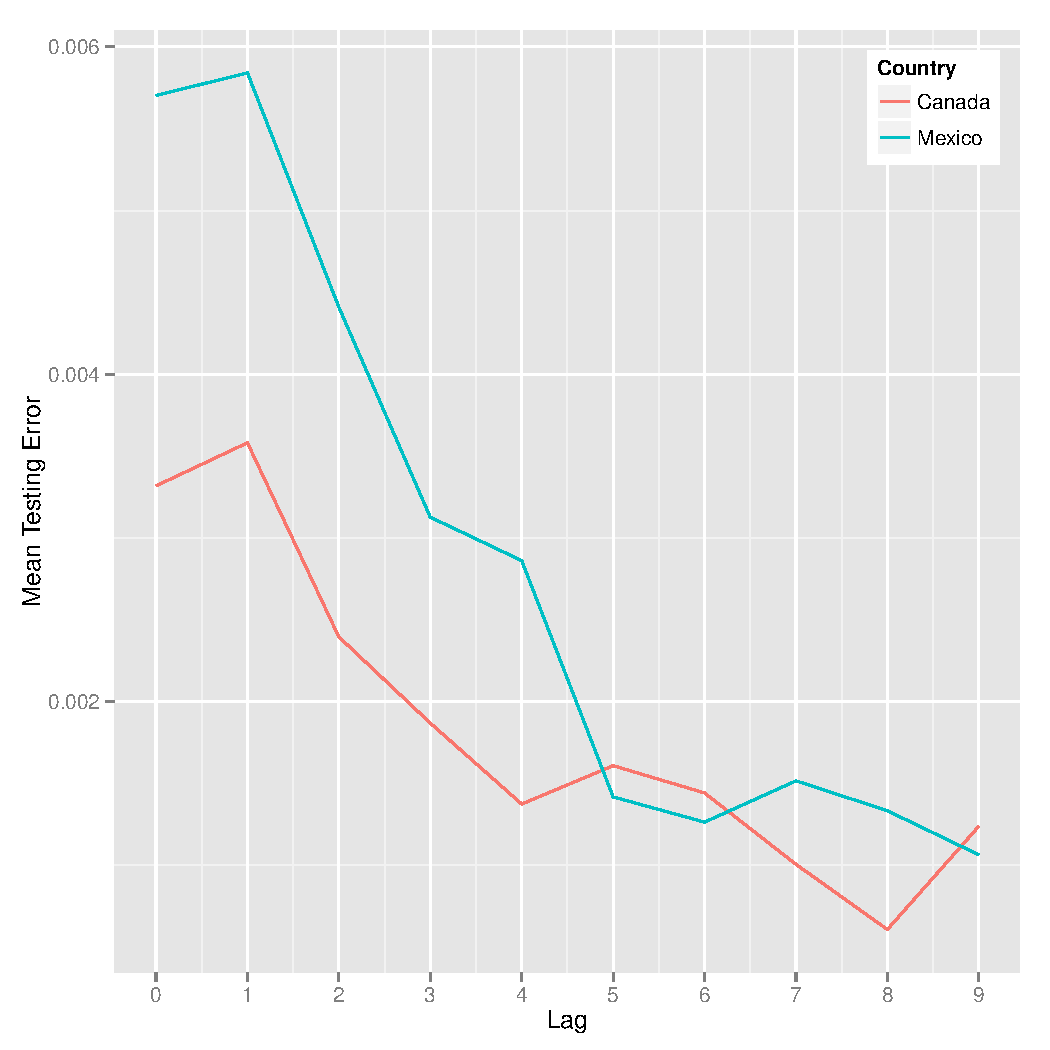
\includegraphics[scale=0.45]{lag1.pdf}
\label{fig:lag1}
\end{figure}

\begin{figure}
\centering
\caption{Model Performance for Various Lags}
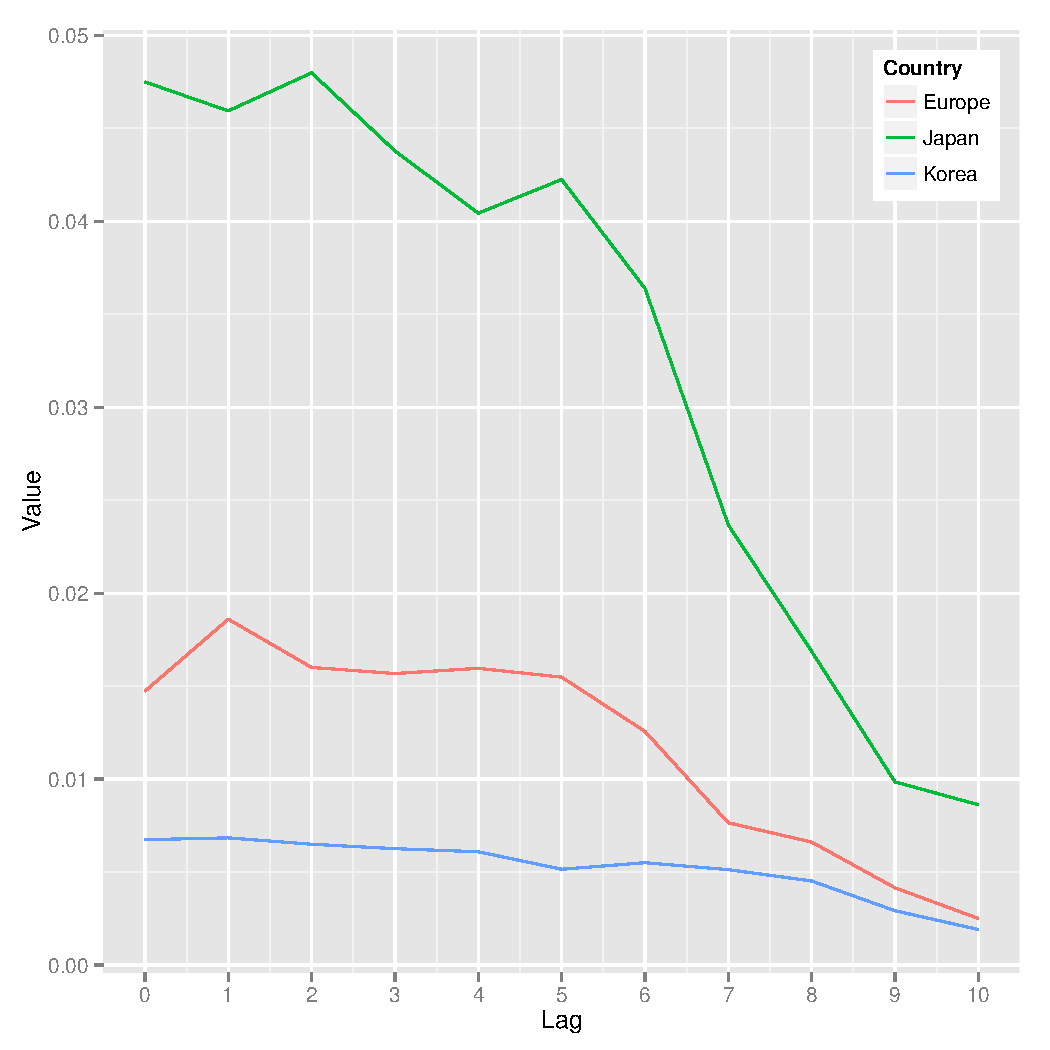
\includegraphics[scale=0.45]{lag2.pdf}
\label{fig:lag2}
\end{figure}

\section{Findings}
     
% hangref environment
\newenvironment{hangref}{\begin{list}{}{\setlength{\itemsep}{0pt}
\setlength{\parsep}{0pt}\setlength{\rightmargin}{0pt}
\setlength{\leftmargin}{+\parindent}
\setlength{\itemindent}{-\parindent}}}{\end{list}}
\section*{REFERENCES}
\begin{hangref}

\item Frankel, J., and A. Rose. 1996.
``A panel project on purchasing power parity: mean reversion within and between countries.''
{\it Journal of International Economics} 40: 209-224.

\item Hsieh, D. 1989
``Testing for Nonlinear Dependence in Daily Foreign Exchange Rate Changes.''
{\it Journal of Business} 62: 329-368.

\item Krugman, P., M. Obstfeld and M.Melitz.  2014.
{\it International Economics: Theory and Policy}. 10th ed.
Upper Saddle River, New Jersey: Pearson Education.

\item Juselius, K. 1995.
``Do purchasing power parity and uncovered interest rate parity hold in the long run? An example of likelihood inference in a multivariate time-series model.''.
{\it Journal of Econometrics} 69: 211-240.

\item Lyons, K.R. and M.D.D. Evans. 2002
``Order Flow and Exchange Rate Dynamics.''
{\it Journal of Political Economy} 110: 170-180

\item Meese, R., and K. Rogoff. 1983.
``Empirical exchange rate models of the seventies: Do they fit out of sample?.'' 
{\it Journal of International Economics} 14: 3-24.

\item Meese, R.A. and A.K. Rose. 1990
``Nonlinear, Nonparametric, Nonessential Exchange Rate Estimation.''
{\it The American Economic Review} 80: 192-196 

\item Obstfeld, M., and A. Taylor. 2003.
``Globalization and capital markets.'' 
{\it Globalization in historical perspective}
University of Chicago Press: 121-188.

\item Wooldridge, J. 2009.
{\it Introductory Econometrics}. 4th Ed.
Mason, Ohio: South-Western Cengage Learning.







\item Panda, C. and V. Narasimhan 2007
``Forecasting exchange rate better with artificial neural network.''
{\it Journal of Policy Modeling} 29: 227-236





\end{hangref}

\clearpage





\end{document}
